\documentclass[preprint,12pt]{elsarticle}

\usepackage{booktabs}
\usepackage{graphicx}
\usepackage{threeparttable}
\usepackage{array}
\usepackage{microtype}

\graphicspath{{./}{../figures/}}

\begin{document}

\section*{Supplementary Material}

\section*{S1. Exploratory maintenance-governance analysis}

The primary manuscript focuses on how denominator choice changes the spatial diagnosis of elevator service continuity. The MTA asset file also identifies whether an elevator is managed by NYCT or by a third party. We retain this information as an exploratory supplementary analysis because management responsibility is not randomly assigned and may correlate with asset age, ownership, maintenance contracts, or reporting practice.

For elevator $i$ in month $t$ and station complex $s$, the primary exploratory model is
\begin{equation}
A_{it} = \beta T_i + \alpha_t + \gamma_s + \varepsilon_{it},
\end{equation}
where $A_{it}$ is MTA-reported availability, $T_i$ indicates third-party management, $\alpha_t$ are month fixed effects, and $\gamma_s$ are station-complex fixed effects. The coefficient is interpreted as an association. We report elevator-clustered and station-complex-clustered standard errors and repeat the comparison within the 13 station complexes containing both management types.

\begin{table}[htbp]
\centering
\caption{Exploratory association between third-party management and MTA-reported elevator availability.}
\label{tab:s1}
\small
\begin{tabular}{lrrrr}
\toprule
Specification & $N$ & Complexes & Coef. (pp) & $p$ \\
\midrule
Month + borough FE; elevator-clustered SE & 45,005 & 133 & -4.43 & 0.0005 \\
Month + complex FE; elevator-clustered SE & 45,005 & 133 & -4.99 & 0.0055 \\
Month + complex FE; complex-clustered SE & 45,005 & 133 & -4.99 & 0.0066 \\
Mixed complexes; elevator-clustered SE & 10,429 & 13 & -4.92 & 0.0063 \\
\bottomrule
\end{tabular}
\end{table}

The point estimate is similar under elevator- and complex-level clustering. It also remains similar when the sample is restricted to mixed-management station complexes. These results are descriptive and are not used to support the manuscript's primary measurement contribution.

\begin{figure}[htbp]
\centering
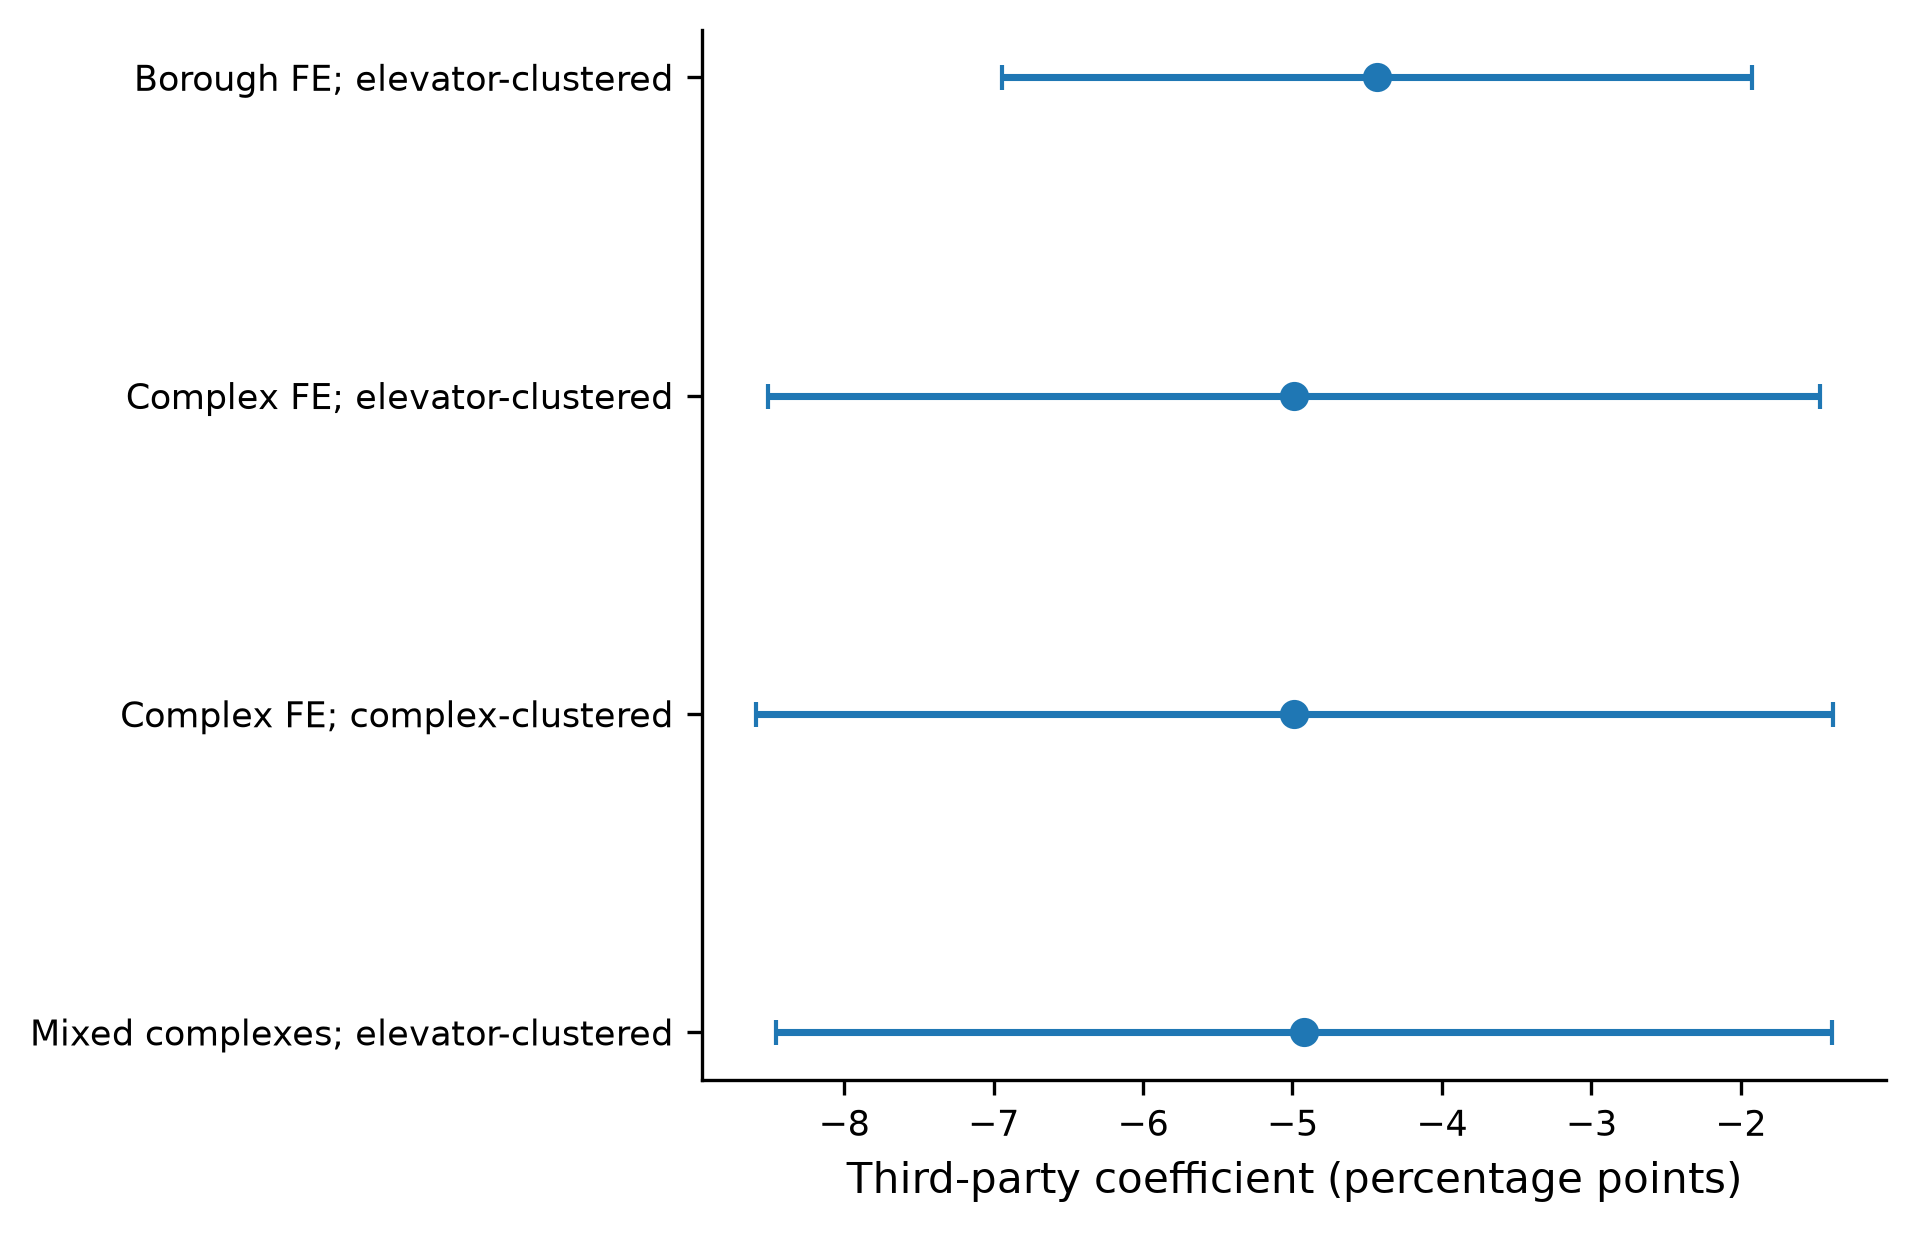
\includegraphics[width=0.88\linewidth]{figS1_management_coefficients.png}
\caption{Third-party-management coefficients and 95\% confidence intervals across exploratory model specifications.}
\label{fig:s1}
\end{figure}

\section*{S2. Calendar-continuity rank persistence}

The main manuscript reports adjacent-year persistence for MTA-reported availability. Calendar continuity shows a similar longitudinal structure. All eleven adjacent-year correlations are positive and statistically significant; the mean Spearman coefficient is 0.525.

\begin{figure}[htbp]
\centering
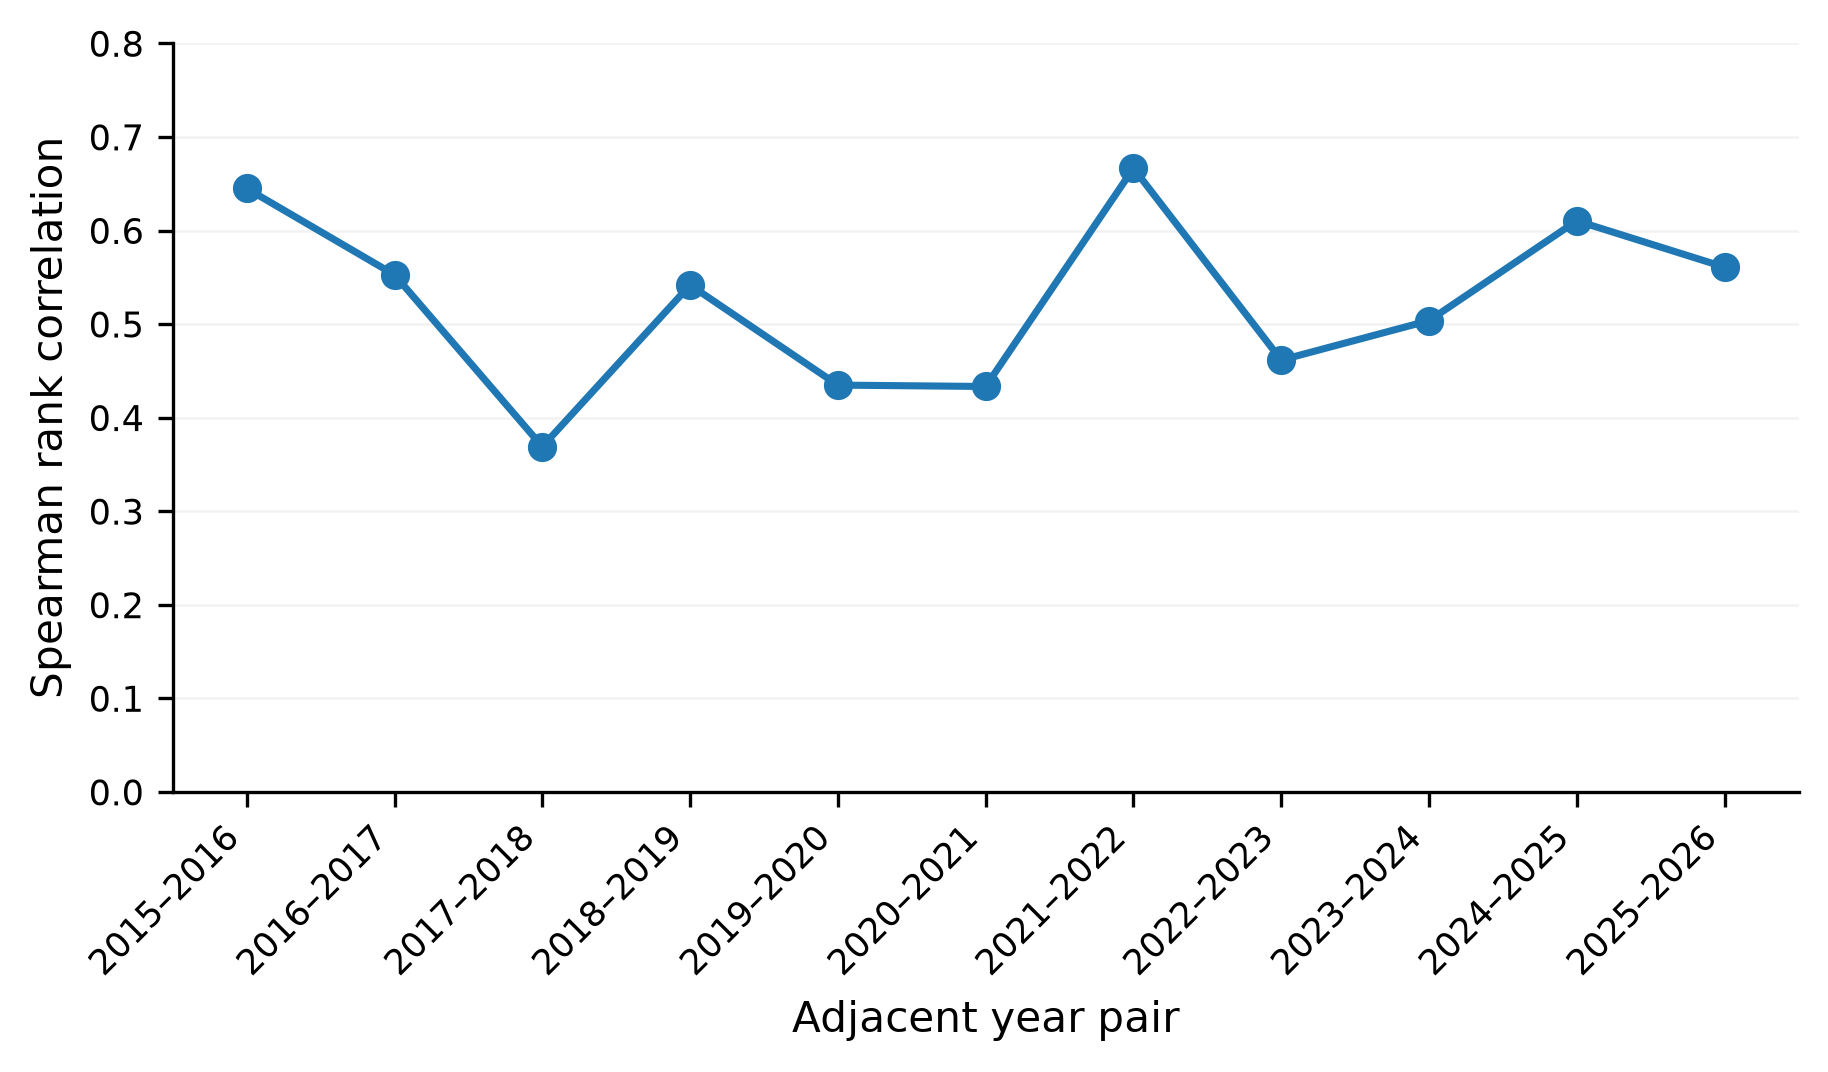
\includegraphics[width=0.92\linewidth]{figS2_calendar_persistence.png}
\caption{Spearman rank correlation of station-complex calendar continuity in adjacent years. Complexes must have at least six observed months in each year.}
\label{fig:s2}
\end{figure}

\section*{S3. Chronicity sensitivity}

Table~\ref{tab:s2} varies the minimum longitudinal-coverage requirement. The association between recurrence under MTA-reported availability and calendar continuity remains between 0.863 and 0.877. Seven complexes remain in the calendar-continuity low-reliability quartile in at least half of observed months, while three retain recurrence increases of at least 0.15.

\begin{table}[htbp]
\centering
\caption{Sensitivity to minimum longitudinal coverage.}
\label{tab:s2}
\small
\begin{tabular}{rrrrr}
\toprule
Minimum months & Complexes & Spearman $\rho$ & $\Delta\geq0.15$ & Continuity recurrence $\geq0.50$ \\
\midrule
24 & 117 & 0.873 & 3 & 7 \\
36 & 113 & 0.877 & 3 & 7 \\
48 & 109 & 0.868 & 3 & 7 \\
60 & 107 & 0.866 & 3 & 7 \\
72 & 105 & 0.863 & 3 & 7 \\
\bottomrule
\end{tabular}
\end{table}

Table~\ref{tab:s3} varies the descriptive low-reliability cut point. The recurrence measures remain positively associated under all three definitions. Cortlandt Street, South Ferry/Whitehall Street, and Court Street/Borough Hall exceed a recurrence increase of 0.15 under the quintile, quartile, and tercile definitions.

\begin{table}[htbp]
\centering
\caption{Sensitivity to the descriptive low-reliability threshold.}
\label{tab:s3}
\small
\begin{tabular}{lrrr}
\toprule
Threshold & Spearman $\rho$ & $\Delta\geq0.15$ complexes & Continuity recurrence $\geq0.50$ \\
\midrule
Bottom quintile & 0.814 & 5 & 3 \\
Bottom quartile & 0.877 & 3 & 7 \\
Bottom tercile & 0.906 & 3 & 19 \\
\bottomrule
\end{tabular}
\end{table}

\end{document}
